\subsection{Introduction}
The whole project is divided into different applications:
\begin{itemize}
	\item Android application built on Unity\\It's the core application of the project that is going to run all the operation required to show and manage the virtual environment shown to the user;
	\item Android application\\It's one of the possible way to read the data from the biosensor.
	\item Pc application\\It's one of the possible way to read the data from the biosensor.
	\item Firebase Server\\Allows the communication between the pc client and the Firebase database.
\end{itemize}

Unfortunately, Unity doesn't offer a simple way to retrieve the data directly from the biosensor and this is the reason that the two alternative application had to be made.
In order to make to communication as simple as possible, it was decided to take advantage of Firebase as a way to store and retrieve data thanks to its database.\\
So, as shown in figure \ref{fig:communication}, the information from the biosensor are read first by a Computer or an Android device and then sent to a Firebase server that stores the values.
\begin{figure}[H]
	\centering
	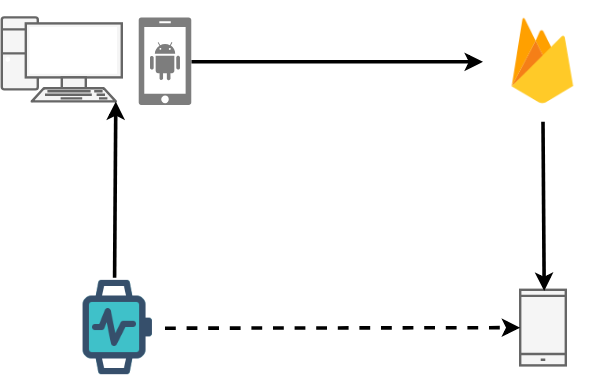
\includegraphics[scale=0.7]{ConnectionDiagram}
	\caption{Diagram that shows how the communication from the biosensor to the smartphone works.}\label{fig:communication}
\end{figure}
One problem that arises with this choice is the need for authentication so that the Unity application is always connected to the right biosensor.\\
To solve this problem, the authentication is done by using QR codes so that the device connected to the biosensor generates a QR code that allows a smartphone to "connect" to it.\\
This solution works with the assumption that the user is near the device that displays the QR code. This is a safe assumption as the biosensor is connected by bluetooth to that device and so the user shouldn't be too far from it.

\subsection{Main Android Application}
Language used: C\#\\
Plugins \& Libraries:
\begin{itemize}
	\item ZXing
	\item Android Runtime Permissions
	\item Speech Engine
	\item FirebaseDatabase
\end{itemize}

\subsubsection{Description}
This is the core of the project and it's split in three parts:
\begin{enumerate}
	\item QR code reader that allows to connect the application to the right "room" where it can retrieve the required data as stated before;
	\item Main menu that contains all of the settings available for the application;
	\item VR application that represent the main component.
\end{enumerate}

In order to accomplish all the task required, the application takes advantages of the functionalities offered by Unity and by the additional libraries to:
\begin{itemize}
	\item Read QR codes thanks to ZXing;
	\item Communicate with Firebase Realtime Database thanks to the respective plugin;
	\item Convert Text-to-Speech thanks to Speech Engine;
	\item Ask the required permissions to execute operations thanks to Android Runtime Permissions;
	\item Track the activity of the microphone thanks to the functions available on Unity.
\end{itemize} 

In order to keep the algorithm as simple as possible, most of them use a counter to decide whether the have to perform an action or not. Usually the algorithm is:
\begin{enumerate}
	\item Read value;
	\item Analyze the value read;
	\item Increase or decrease the counter based on the analysis;
	\item Check whether the counter is greater or lower than a set threshold;
	\item Perform the action if the threshold was exceeded.
\end{enumerate}
This system is used in many algorithm (as shown in the next section) as a way to manage the environment and decide which action should be performed.
\subsubsection{Algorithm design}
\begin{figure}[H]
	\centering
	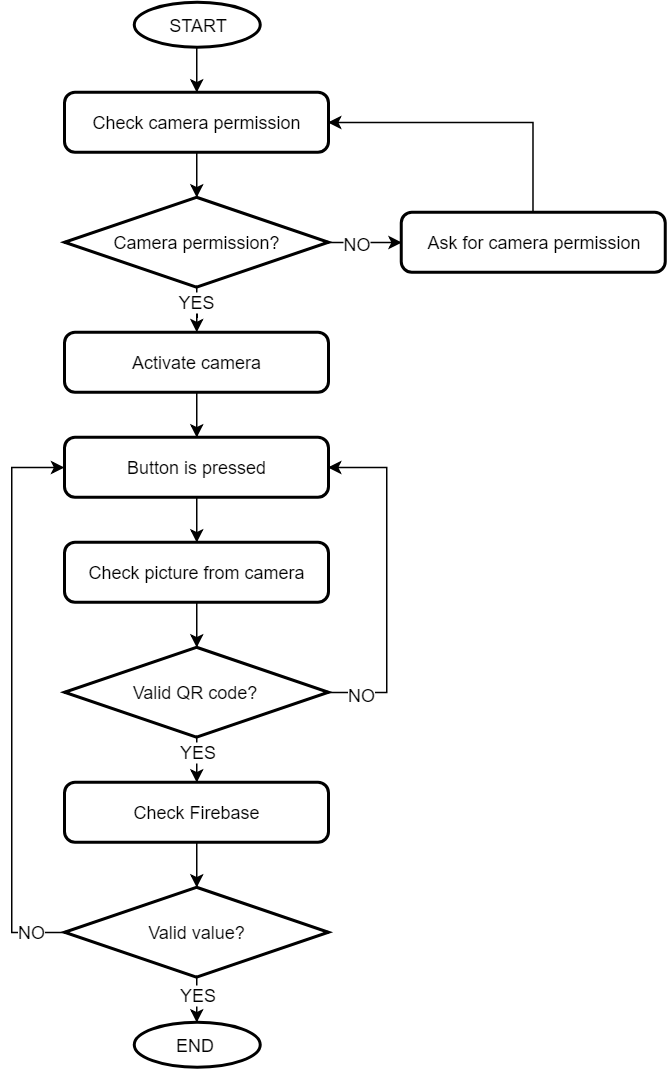
\includegraphics[scale=0.5]{AndroidQRCode}
	\caption{Flowchart that describes how the connection to the right "room" in the Firebase server works}
\end{figure}

\begin{figure}[H]
	\centering
	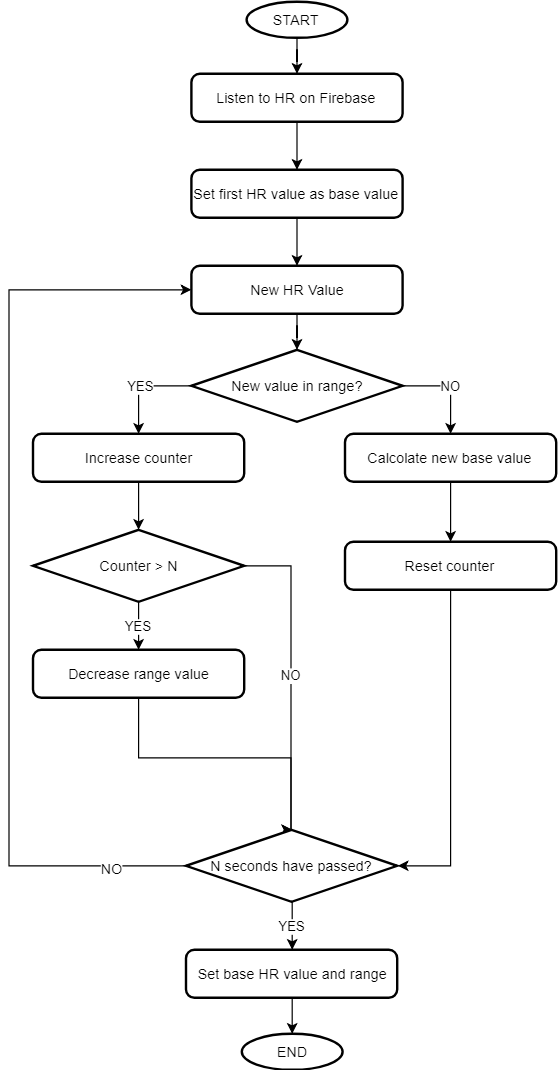
\includegraphics[scale=0.55]{BaseValue}
	\caption{Flowchart that describes how the search of the base value for HR and GSR works. The two operations are executed in two different coroutines.}
\end{figure}

\begin{figure}[H]
	\centering
	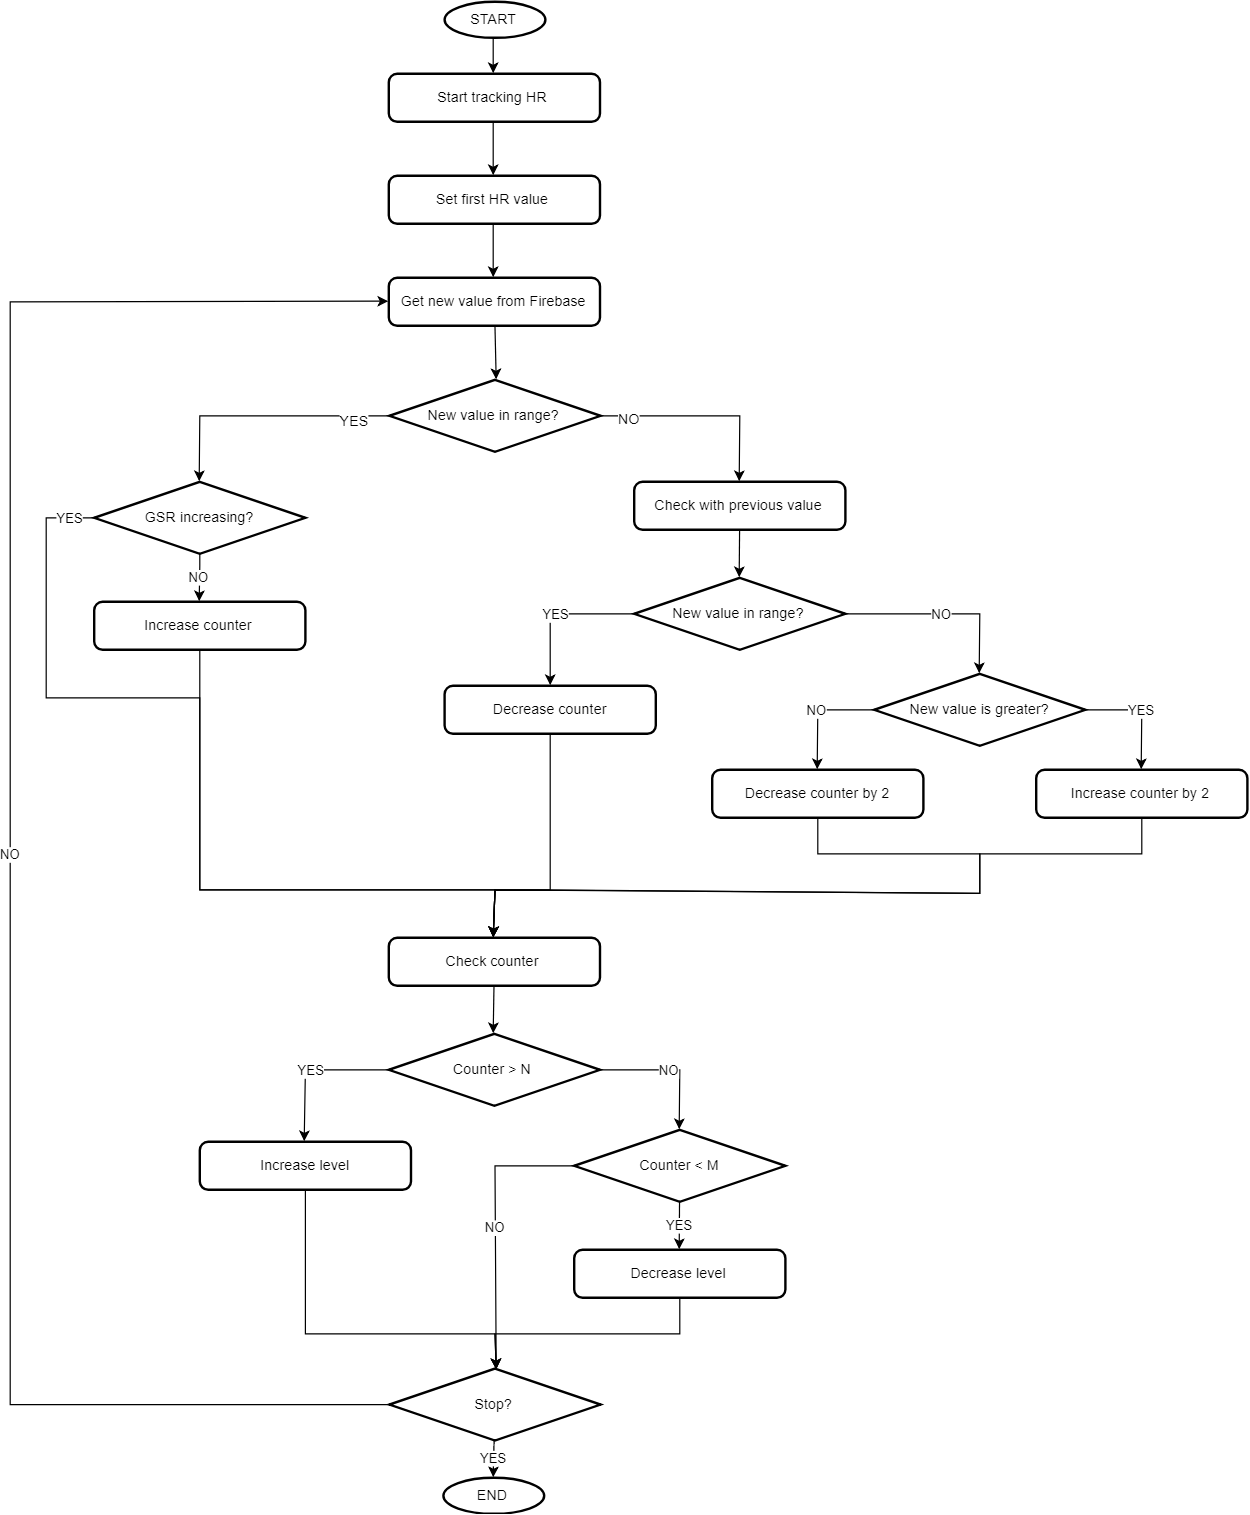
\includegraphics[scale=0.38]{Tracking}
	\caption{Flowchart that describes how the HR and GSR are used to determine whether to increase the level or not.}
\end{figure}

\begin{figure}[H]
	\centering
	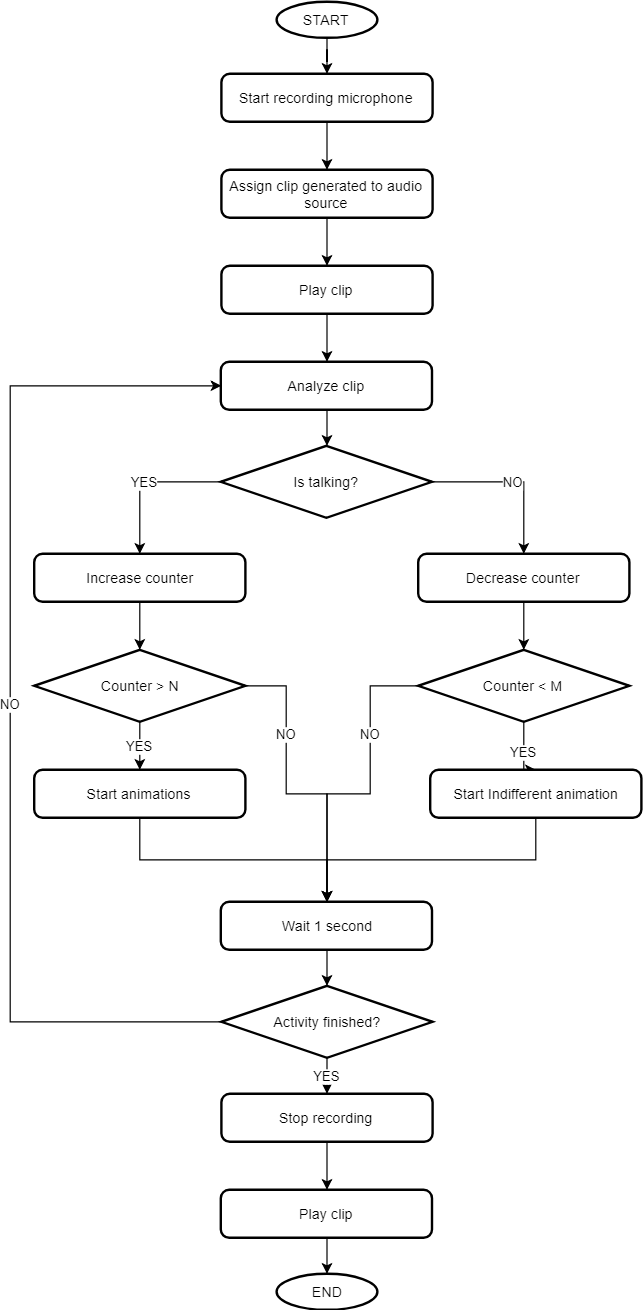
\includegraphics[scale=0.45]{Microphone}
	\caption{Flowchart that describes how the microphone is used to determine whether the animations should be played or not.}
\end{figure}

\begin{figure}[H]
	\centering
	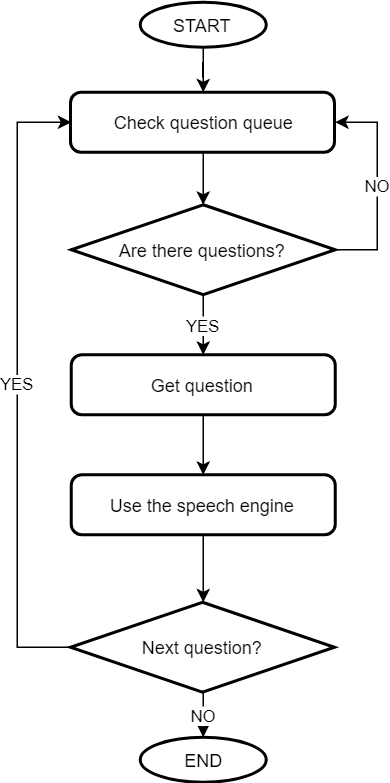
\includegraphics[scale=0.60]{QuestionVoice}
	\caption{Flowchart that describes how question system works when the user doesn't want to get the questions from the audience.}
\end{figure}

\begin{figure}[H]
	\centering
	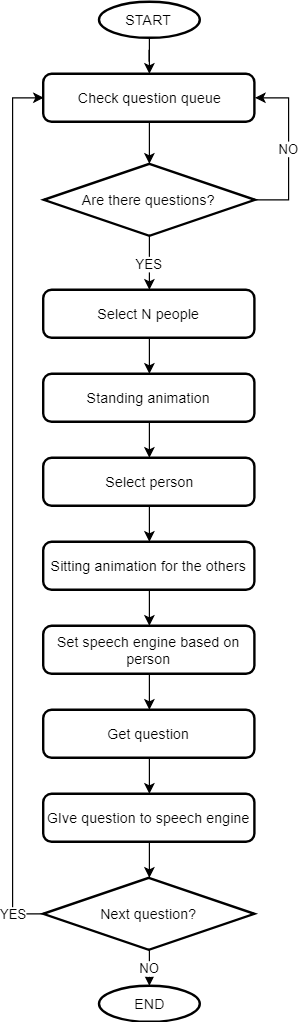
\includegraphics[scale=0.58]{QuestionAudience}
	\caption{Flowchart that describes how question system works when the user want to get the questions from the audience.}
\end{figure}

\subsection{Computer Client}
Language used: Java\\
Plugins:
\begin{itemize}
	\item ZXing
	\item JavaFX
\end{itemize}

\subsubsection{Description}
The computer client main task is to retrieve data from the Empatica E4 and send the values to the Firebase server. In order to do this, it communicates with E4 streaming server, an application that allows to forward realtime data of multiple Empatica E4 devices to multiple TCP socket connections.\\
The E4 Streaming server works through a message protocol where client request are in the following format:
\begin{center}
	COMMAND ARGUMENT\_LIST
\end{center}
Messages from server containing responses to commands are in the following format
\begin{center}
	COMMAND ARGUMENT\_LIST
\end{center}
Messages from server containing data from device are in the following format
\begin{center}
	STREAM\_TYPE TIMESTAMP DATA
\end{center}
The commands used from the client are:
\begin{itemize}
	\item device\_list\\
	requests the list of Empatica E4 devices to the E4 Streaming server
	\item device\_connect DEVICE\_ID\\
	sends a connection request to a specific device
	\item device\_subscribe STREAM STATUS\\
	start or stop receiving data from a given stream.
	\item device\_disconnect\\
	sends a device disconnection request
\end{itemize}
\pagebreak
\subsubsection{Algorithm design}
\begin{figure}[H]
	\centering
	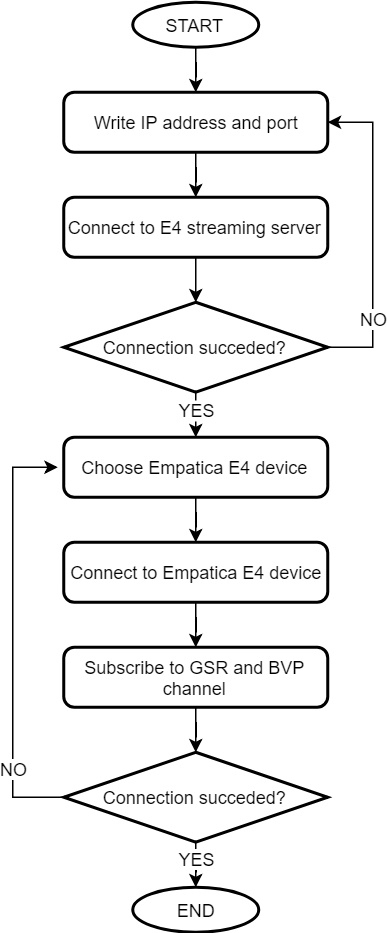
\includegraphics[scale=0.5]{BiosensorConnectDiagram}
	\caption{Flowchart that describes how the connection to the Empatica E4 device works}
\end{figure}

\begin{figure}[H]
	\centering
	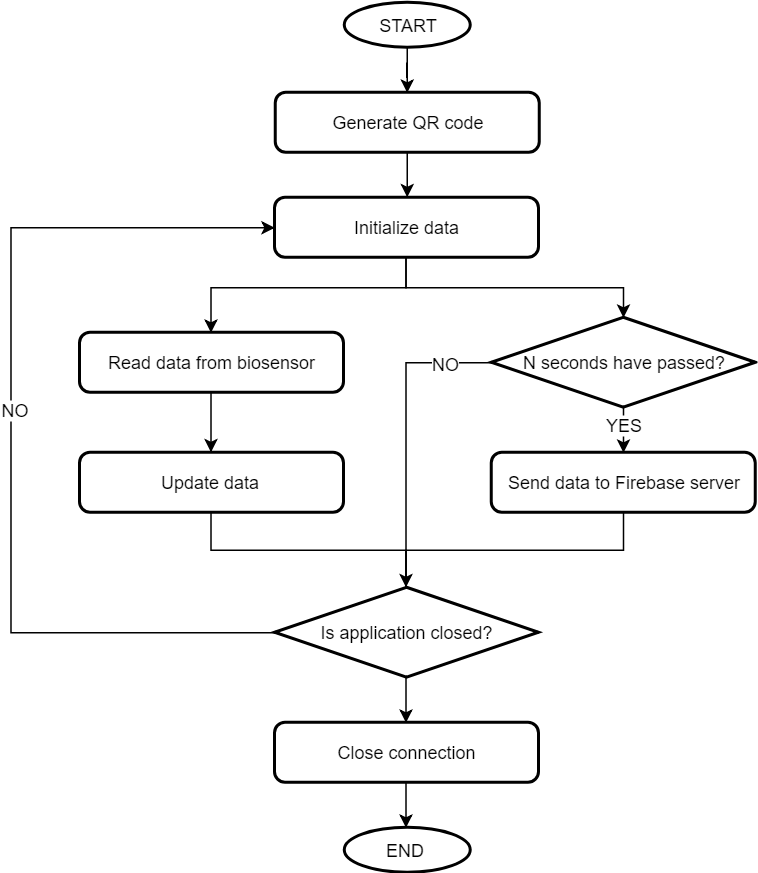
\includegraphics[scale=0.55]{BiosensorDataDiagram}
	\caption{Flowchart that describes how the client retrieve data from the Empatica E4 after the connection has been established}
\end{figure}
\pagebreak

\subsection{Firebase server}
Language used: Javascript

\subsubsection{Description}
Firebase is a platform that offers the possibility develop web application easily. It was chosen as the backend for this project because of its ease of use.\\
The main objective of the Firebase application is to store the data retrieved from the biosensor and then send them when requested.\\
The services used on Firebase are:
\begin{itemize}
	\item Realtime Database.
	\item Cloud functions;
\end{itemize}
The Realtime Database is a NoSQL database were data is stored as JSON. It is used to store the value read by the biosensor and the questions that have to be sent to the mobile application.
\begin{figure}[H]
	\centering
	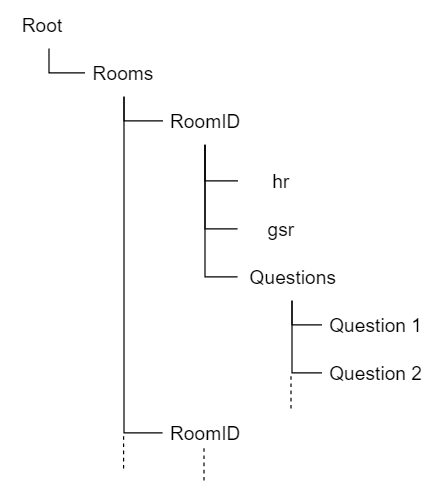
\includegraphics[scale=0.7]{DatabaseStructure}
	\caption{Structure of the Realtime Database}
\end{figure}
Cloud functions are used in order to let the PC client access the database. The Cloud functions are tasks that can be triggered by HTTP requests. The values required are sent as a JSON string in the body of the request.
\begin{itemize}
	\item createRoom: creates a room with the given room code;
	\item updateValues: update the values of the hr and gsr stored in the given room;
	\item addQuestion: add a question to the list in the given room;
	\item removeRoom: Closes the room with the given room code.
\end{itemize}

\subsection{Android Application}
Language used: Java
Plugins \& Libraries:
\begin{itemize}
	\item ZXing
	\item AndroidImagePopup
	\item FirebaseDatabase
	\item Empalink
\end{itemize}

\subsubsection{Description}
The Android application main task is to retrieve data from the Empatica E4 and send the values to the Firebase Database. in order to do this, it communicates with the biosensor thanks to the Empalink library developed by Empatica that allows to read the data directly from the Empatica E4 without the need of another application (unlike the pc application that needs the E4 streaming server.

\subsubsection{Algorithm design}
\begin{figure}[H]
	\centering
	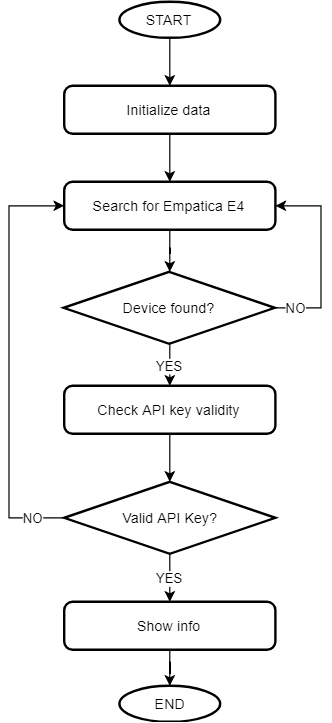
\includegraphics[scale=0.65]{BiosensorConnectDiagramAndroid}
	\caption{Flowchart that describes how the client connects to the Empatica E4 biosensor}
\end{figure}

\begin{figure}[H]
	\centering
	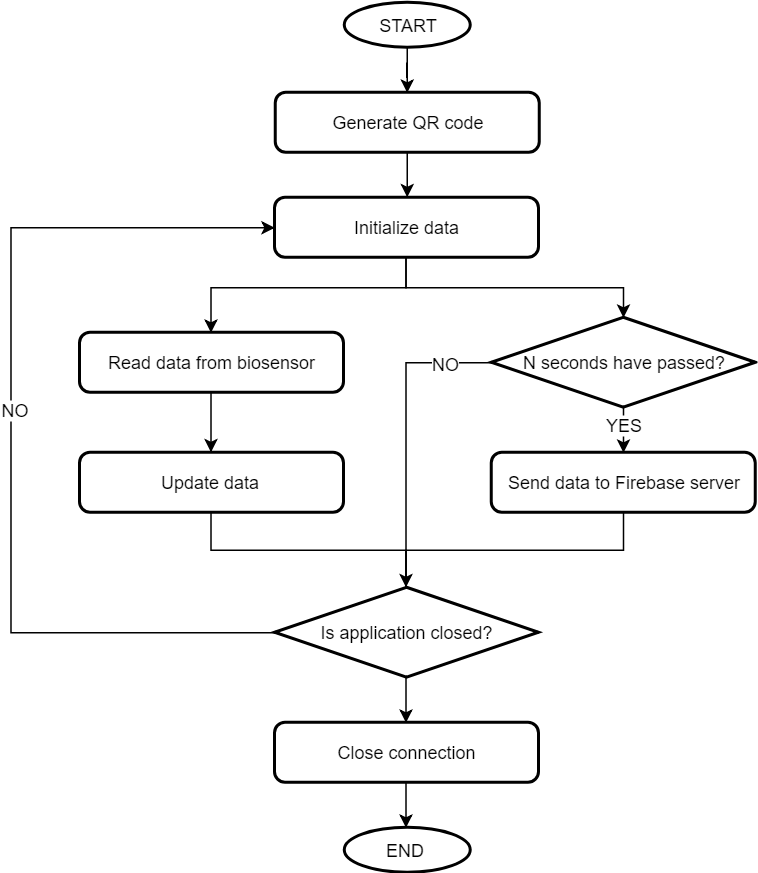
\includegraphics[scale=0.55]{BiosensorDataDiagram}
	\caption{Flowchart that describes how the client retrieve data from the Empatica E4 after the connection has been established (same as the pc client)}
\end{figure}